\chapter{Discussion}
By applying a local approach to building the configuration space, the riddles are starting to become solvable in an acceptable timeframe.
Still, the time it takes to solve a riddle can vary strongly depending on the number of objects, their start configuration and their shape. Furthermore, there are still some unsolved problems in general and depending on the used implementation

\section{General Problems}
\subsection{Rotation Steps}
\begin{figure}[H]
\centering
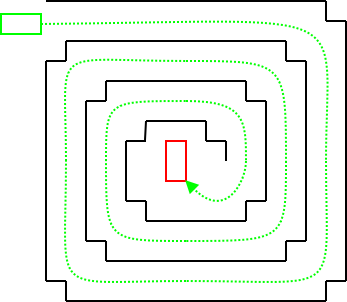
\includegraphics[scale=0.5]{endlessRot}
\caption{Figure showing a main object (green) with a spiral like obstacle (black) and a target area (red).}
\label{rotFigure}
\end{figure}
As each object can be rotated a total 360° to get back to its starting orientation, the rotation dimension is finite. In figure \ref{rotFigure} it can be seen that the object can nevertheless be moved and rotated more than 360°. What happens is that as soon as the rotation would be bigger than 360° the rotation is set back to 0°. This can be done due to the fact that the collision sets containing an object with the configuration $(x_1 , y_1, \phi_1)$ is equal to that of $(x_1, y_1, \phi_1 + 360)$.\\
The problem is, that for algorithm P with points lists convex hulls are needed in order to check for collision of moving objects. But the objects hull including the rotation axis would be non-convex as the object would be moved along the rotation axis in a sinuid fashion. Therefore the rotation is done on a grid to build a stack of hyperplanes containing the configuration of each object. For every rotation a new hyperplane is created with only the moving objects rotation changed.\\
The downside to that is, that in order to build a stack, there is the need to define a stepsize in which to move up and down the stack and change the rotation. This leads to another scaling factor which needs to be set so that adequate accuracy can be achieved. One has to choose either less accuracy for less calculations or more calculations for higher accuracy.

\subsection{Missing Heuristic}
The heuristik used in all algorithms for A$^\star$ is the distance beetween the current and the target configuration for the main object. For all other object there is no heuristik. Therefore it is not possible after moving, them to tell if the configuration improved or not. So to find a solution, the obstacles need to be moved at random until the heuristik for the main object improves meaning the distance decreased. This can lead to the same effect as shown in \ref{subsec:counterheuristic}.\\
Developing a good heuristic for the obstacles is not that easy on the other hand, due to the fact that one can not easily tell which direction those objects should take to free the way.\\
An idea would be to work with a field generated by putting a two-dimensional gauss function on every obstacle and a sink at the target. The heuristik could then be calculated as the sum of all obstacle gauss functions and the sink function. The higher the value, the worse the positioning of obstacles. \\
Another maybe to simple approach would be to prefer obstacles in the direct line beetween main object and target to be moved. This can lead to problems if the way to the target requires moving in a half-circle way. To refine this it could also be possible to calculate the way to the target without obstacles in the riddle, then mark all obstacles on the path and try to move them away until the path is cleared.

\section{Problems with Point List Implementation}
%\subsection{Invisible Plains}
An invisible plain is a plain extending from the vector of one object between two of its points. This plain splits the search space in two parts. Due to the fact, that this effect is used to split the space in cells, which is needed for obtaining nodes in the search graph, changes to these plains affect the graph.\\
\begin{figure}[H]
\centering
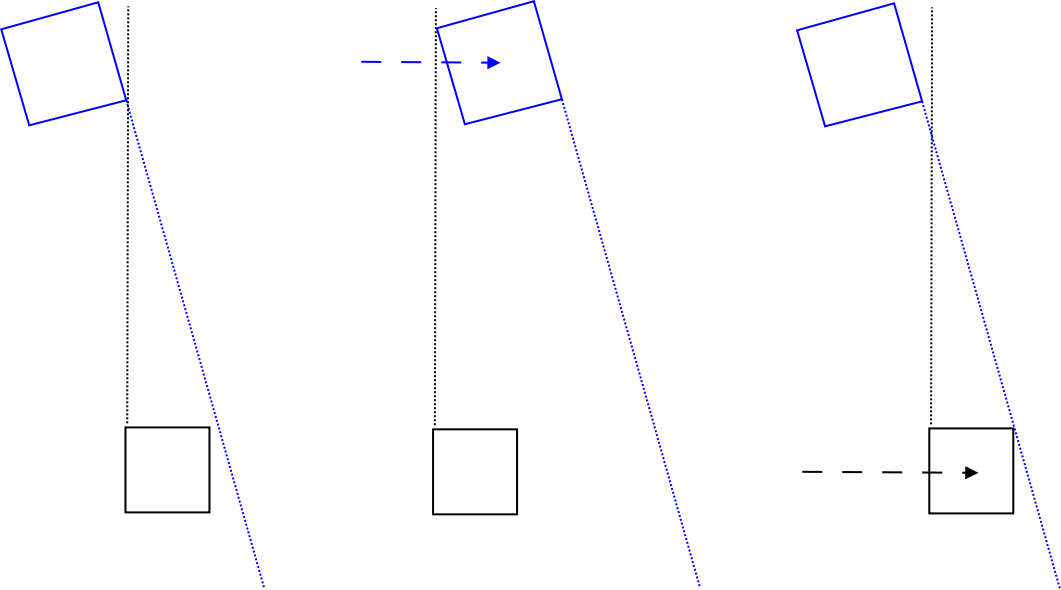
\includegraphics[scale=0.3]{ghostplanes}
\caption{Two objects with interfering planes}
\end{figure}
 This example shows how the black object $O_1$ dictates the cell border for the blue object $O_2$ on the right. If $O_2$ is moved over the border, it now takes over the cell border for object  $O_1$. Without a given heuristic which object is better to be moved to the right, this will end in alternating movements for both objects.\\
But if  $O_1$ is the main object, which has a target on the right, the heuristic would tell the search algorithm that the point with $O_1$ beeing right of  $O_2$ is the better point, and search from there on further, meaning $O_1$ beeing moved over the right cell border.

\section{Problems with Function List Implementation}
%\subsection{Vertical Lines}
Due to the nature of a function, vertical lines cannot be represented. This leads to the rule that all objects in the riddle cannot have a vertical line even after rotating. 
To still be able to draw an object with a vertical line, a function is defined with a very high gradient and setting the starting point at the x-coordinate of the vertical line. This leads to a near vertical line, that is still a function, and as such can be used in the calculations.\\
The drawback is clearly the loss of precision. How strong this loss is depends on the initial gradiant one gives the function. A seemingly good idea would be to use the max value of the variables used in calculations (e.g. double = $1.7977 \cdot 10^{308}$ ). But if this is done without being sure that this value will never be used in a way, such that the solution of a calculation could be greater than the gradiant, an overflow would be possible.\\
Thus, a value needs to be found that leaves enough room for calculations and still keeps the precision loss as small as possible. The exact number depends on the system the algorithm is used in. Also one needs to cap the gradiant after each rotation, so that it does not exceed the given max value.


